\section{3D Printing BaSO\textsubscript{4}\label{sec:methodology:3dPrintingBaSO4}}

The custom-made PLA with BaSO$_4$ (see~\fullref{sec:methodology:extrudingBaSO4}) was 3D printed to create samples for imaging and mechanical testing.

\subsection{Nozzle Replacement\label{sec:methodology:3dPrintingBaSO4:nozzleReplacement}}

When printing PLA with barium sulfate, a standard 0.4mm stainless steel nozzle was initially used. This led to regular clogging of the hotend. It was hypothesized that if larger barium sulfate pieces were inhibiting the flow of material, a larger nozzle may help resolve this clogging. Additionally, abrasive filaments inflict substantial damage on a nozzle, and a wear resistant nozzle is thus recommended~\cite{RefWorks:RefID:500-2019abrasive}.

As a result, the standard 0.4 stainless steel nozzle was replaced with a 0.6mm cold-hardened nozzle as shown in Figure~\ref{fig:methodology:3dPrintingBaSO4:differentNozzles}.

\begin{figure}[h!]
        \centering
        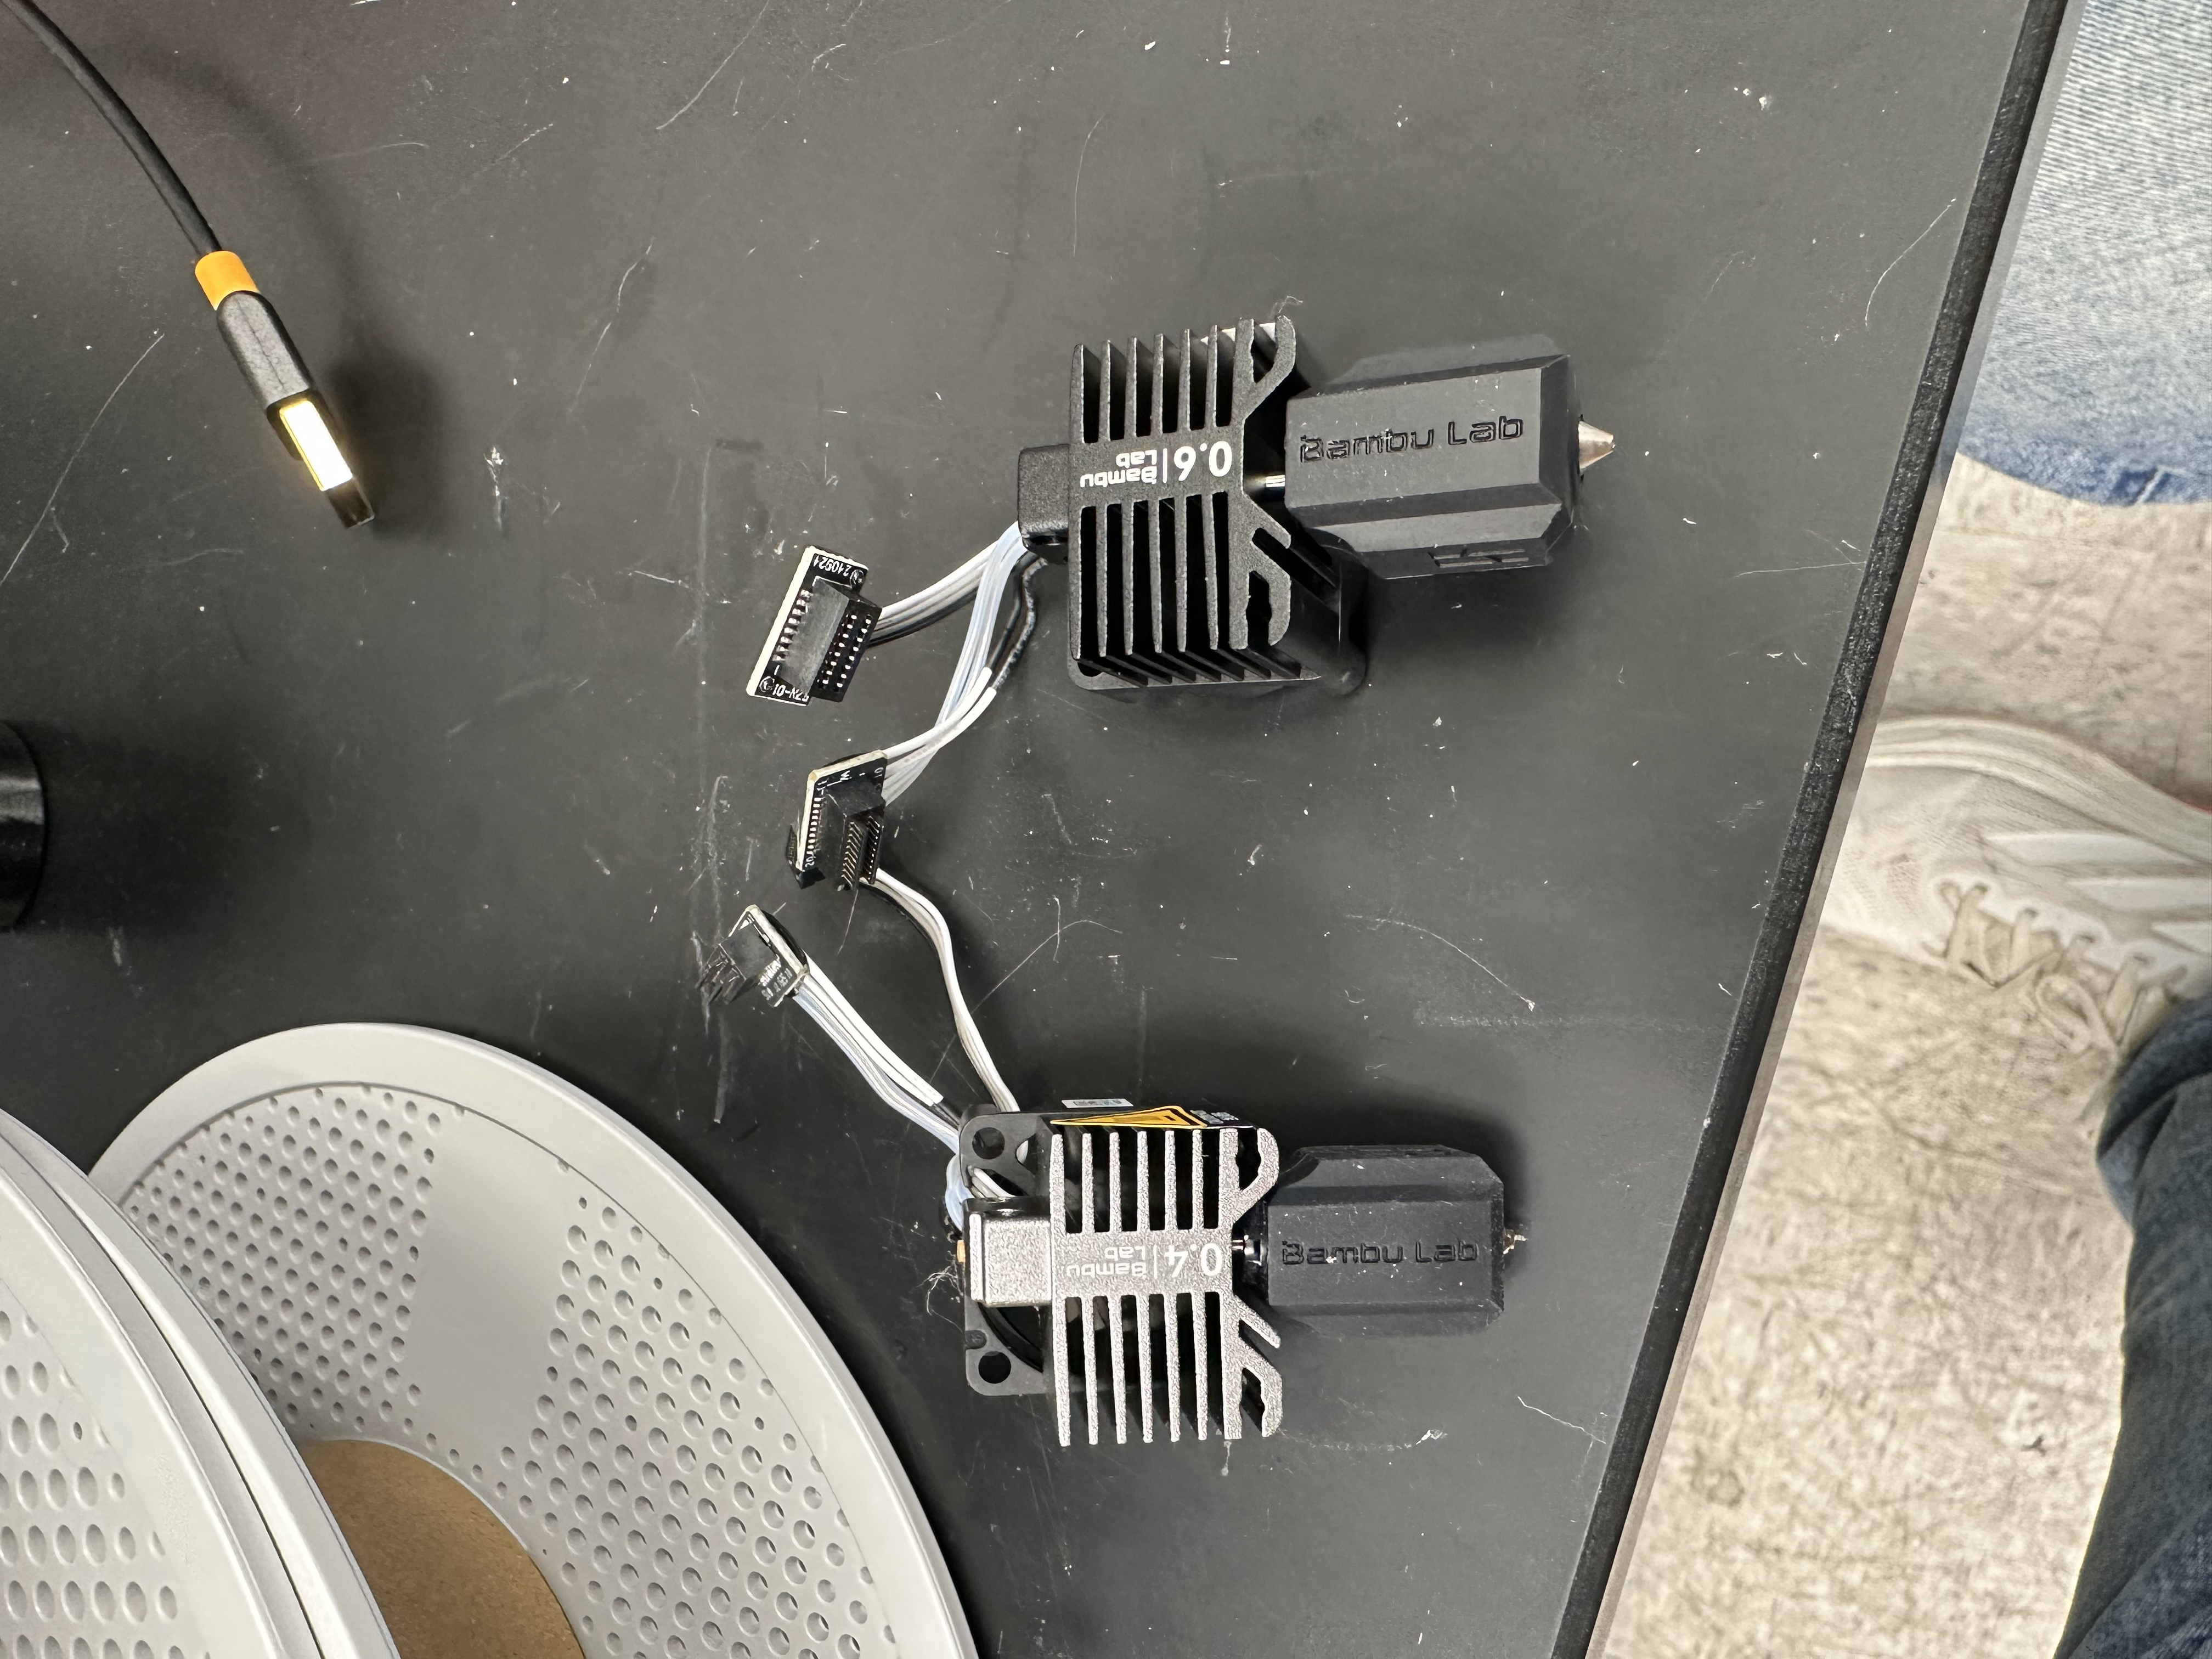
\includegraphics[width=0.5\linewidth]{../figs/methodology/3dPrintingBaSO4/different_nozzles.png}
        \caption{0.4mm stainless steel hotend assembly (left) vs 0.6mm cold-hardened steel hotend assembly (right).}
        \label{fig:methodology:3dPrintingBaSO4:differentNozzles}
\end{figure}

This nozzle replacement immediately resolved the noticed clogging when 3D printing.

\subsection{Optimizing Printing Parameters\label{sec:methodology:3dPrintingBaSO4:printingParameters}}

\paragraph*{Guess-and-Check Approach}
Because the PLA/BaSO\textsubscript{4} filaments were predominantly PLA, the generic PLA presets were initially used to establish printing parameters. This led to underextrusion and clogging, so various parameters were changed based on best guesses. These included print bed temperature, flow rate, and nozzle temperature. This guess-and-check approach yielded usable but unreliable printing parameters.

\paragraph*{Bambu Marble}
In Bambu Studio, Bambu Marble filament was then selected as a base material rather than generic PLA. Bambu Marble is a filament with marble embedded inside, and it was hypothesized that stone-embedded filaments (both marble or barium sulfate) may use similar printing parameters.

This solution worked well and immediately led to more optimal printing. Filaments with higher barium sulfate concentrations still exhibited clogging at these parameters, so the nozzle temperature was raised in 5\textcelsius ~increments to decrease the viscosity of the filament.

Due to limited material, formal calibrations such as Flow Dynamics and Flow Rate calibrations, were not performed on these filaments. Instead, a calibration cube, as shown in Figure~\ref{fig:methodology:3dPrintingBaSO4:calibrationCube}, was printed to ensure proper printing parameters.

\begin{figure}[h!]
        \centering
        \includegraphics[width=0.5\linewidth]{../figs/methodology/3dPrintingBaSO4/calibration_cube.png}
        \caption{Calibration cube used to test barium sulfate filaments.}
        \label{fig:methodology:3dPrintingBaSO4:calibrationCube}
\end{figure}

Final printing parameters and discussion of these findings can be found in~\fullref{sec:results:3dPrintingBaSO4:printingParameters} and~\fullref{sec:discussion:3dPrintingBaSO4:printingParameters} respectively.
